\chapter{Introduction}
\pagenumbering{arabic}
\pagestyle{plain}

\section{DNA damage and its consequences}

The impeccable preservation of DNA is surely one of the most essential requirements for cellular viability. On a single day DNA accumulates on average $\sim\text{10}^\text{5}$ damages per cell, which can be grouped into three different categories \cite{Hoeijmakers2009}. First, DNA constantly undergoes spontaneous unspecific reactions (mostly hydrolysis) that cause deamination and create abasic sites in an aqueous solution \cite{Lindahl1993,Lhomme1999}. Second, the most common type of DNA damage originates from the cellular metabolism, which produces various types of reactive oxygen and nitrogen species,lipid peroxidation products, endogenous alkylating agents, estrogen and cholesterol metabolites, and reactive carbonyl species. The subsequent molecular distortions range from several kinds of single-strand breaks to various oxidative base and sugar products \cite{DeBont2004,Sander2005}. And third, DNA damages that are caused by external physical or chemical agents like sunlight, which induces approximately 30,000 pyrimidine dimers per hour in each exposed keratinocyte \cite{Luijsterburg2010}.\\        
The consequences for the cellular viability that arise from the diversity of DNA lesions are essentially twofold. Either, the inflicted chromosomal aberrations are not recognized or bypassed by the DNA repair machinery and thus persist in the genetic Code \cite{Hoeijmakers2009}. These mutations can activate oncogenes or inactivate tumour suppressor genes, which is equivalent to an increase in the cell's cancer risk level \cite{Bartek2007}. Or, alternatively, the damage is so strong that essential cellular processes such as transcription or replication are impaired. This is usually the case for interstrand cross-links or double-strand breaks induced by ionizing irradiation. The occurrence of such lesions leads to accelerated cell death, which particularly in proliferative tissues promotes symptoms of premature ageing \cite{Marteijn2014}. Depending on the location and number of lesions, the cell type, stage in the cell cycle and differentiation both outcomes can happen concurrently. In fact, both cell fates are directly linked considering that damage-induced cell-death protects the body from cancer \cite{Hoeijmakers2009}.            

\paragraph{DNA damage response}    
DNA is the only known biological macromolecule, which cannot be replaced if parts of it are destroyed. This has the inevitable consequence that any mutation that escapes cell-death will persist over the lifetime of the cell \cite{Hoeijmakers2009,Marteijn2014}. For this reason, cells evolved an elaborate genomic maintenance apparatus, the DNA damage response (DDR), that keeps DNA damage under control \cite{Ciccia2010}. The DDR system not only includes various DNA-damage sensors and the enzyme machinery catalysing the individual repair reactions. It also  involves a prophylaxis mechanism through tanning; it regulates a range of downstream mediators and signalling molecules that control cell cycle state and cell fate and most importantly it comprises a number of complementary repair systems, each of which responsible for a specific type of damage \cite{Ciccia2010,Marteijn2014}. Subtle chemical alterations like oxidative lesions and alkylation products are removed by base-excision repair (BER) \cite{Lindahl2000,Caldecott2008}. More complex lesions like interstrand crosslinks (ICLs) or helix distorting lesions are repaired by ICL repair or nucleotide excision repair, respectively \cite{Moldovan2009,Hoeijmakers2009}. Entire cuts of the DNA are processed either by nonhomologous end joining (NHEJ) or homologous repair (HR) \cite{Caldecott2008,West2003}. 

\paragraph{Spatiotemporal regulation of DNA repair} For all repair mechanisms their spatiotemporal regulation follows the general organization of chromatin-associated processes: a) detection of the target site (\textit{e.g.} a DNA lesion) b) assembly of the repair components to a multi-protein complex at the DNA and c) catalysis of an enzymatic reaction with the DNA as a substrate \cite{Hoeijmakers:2001:Nature:11357144,Gillet:2006:Chem-Rev:16464005,Dinant:2009:J-Cell-Biol:19332890,Luijsterburg2010}. Of much interest is thereby the role of the assembly phase, which was, until recently, understood as a sequential, cooperative recruitment of components \cite{Volker2001}. A competing perception considers the complex formation as a combined process of randomly diffusing and rapidly exchanging components \cite{Luijsterburg2010}. This is supported by experimental evidence for DNA repair but also transcription initiation showing that dissociation and rebinding for the constituents of the respective complexes occur on the seconds to minutes time scale \cite{Vermeulen2011,Stasevich2011}. Similar findings are reported for the clustering of RNA polymerases and for replication, with the exception of stably bound Mcm proteins that determine licensed replication origins \cite{Kuipers2011,Sonneville2012}. However, it remains poorly understood how the dynamic interplay of these multi-protein machineries effects the formation of essential system properties like fidelity, timing and robustness. 




\section{NER as a model system for chromatin-associated processes}
\label{sec:NERexperiments}
To gain more insight into the assembly and functioning of protein complexes we have studied the mammalian nucleotide excision repair (NER) pathway. NER is involved in the elimination of a wide range of structurally unrelated DNA lesions, including cyclobutane-pyrimidine dimers (CPDs) and 6-4 pyrimidine-pyrimidone photoproducts (6-4PPs), both induced by ultraviolet (UV) light; various bulky chemical adducts (man-made and natural); intrastrand crosslinks caused by drugs such as cisplatin; and ROS-generated cyclopurines \cite{Marteijn2014}. Consequently, the NER machinery is in itself a composition of intertwined repair mechanisms, which give rise to an exceptional clinical heterogeneity associated with the impairment of NER components.


\paragraph{Molecular mechanism of NER}
The process of damage detection by NER is distinguished into transcription-coupled NER (TC-NER) \cite{Sugasawa:2005:Cell:15882621,Gillet:2006:Chem-Rev:16464005}, where bulky DNA adducts block the transcription machinery and global genome NER (GG-NER) where the same adducts are eliminated throughout the whole genome \cite{Fousteri2008}. In this work we will focus on GG-NER whose core repair factors are all identified and intensively studied. For GG-NER the initial lesion detection is performed by XPC \cite{Sugasawa:1998:Mol-Cell:9734359,Volker2001}. The binding of XPC promotes the association of the TFIIH (transcription initiation factor IIH) complex \cite{Yokoi:2000:J-Biol-Chem:10734143,Riedl2003,Volker2001}. TFIIH consists of 10 components out of which the subunits XPB and XPD have helicase activity with opposite polarity \cite{Tapias2004,Compe2012}. Upon DNA unwinding XPA can bind to altered nucleotides on the damaged single strand whereas the replication protein A (RPA) protects the undamaged strand. Alongside the endonucleases XPG and ERCC1/XPF excise approximately 30 nucleotides around the lesion \cite{Evans1997,deLaat:1998:Genes-Dev:9716411,Wakasugi:1997:J-Biol-Chem:9188507,Park:2006:FEBS-J:16623697,Camenisch:2006:Nat-Struct-Mol-Biol:16491090}. Subsequently, the proliferating cell nuclear antigen (PCNA) is loading the polymerase $\delta$, which refills single-strand DNA gap \cite{Hoeijmakers:2001:Nature:11357144,Essers2005,Moser:2007:Mol-Cell:17643379}. After ligation by LigIII-XRCCI the DNA strand is then rechromatinised by CAF1, which completes the repair process \cite{Green:2003:EMBO-J:14517254,Polo2006} (see Figure \textbf{tbm} for comparison). 

\begin{figure}[htbp]
	\begin{center}
		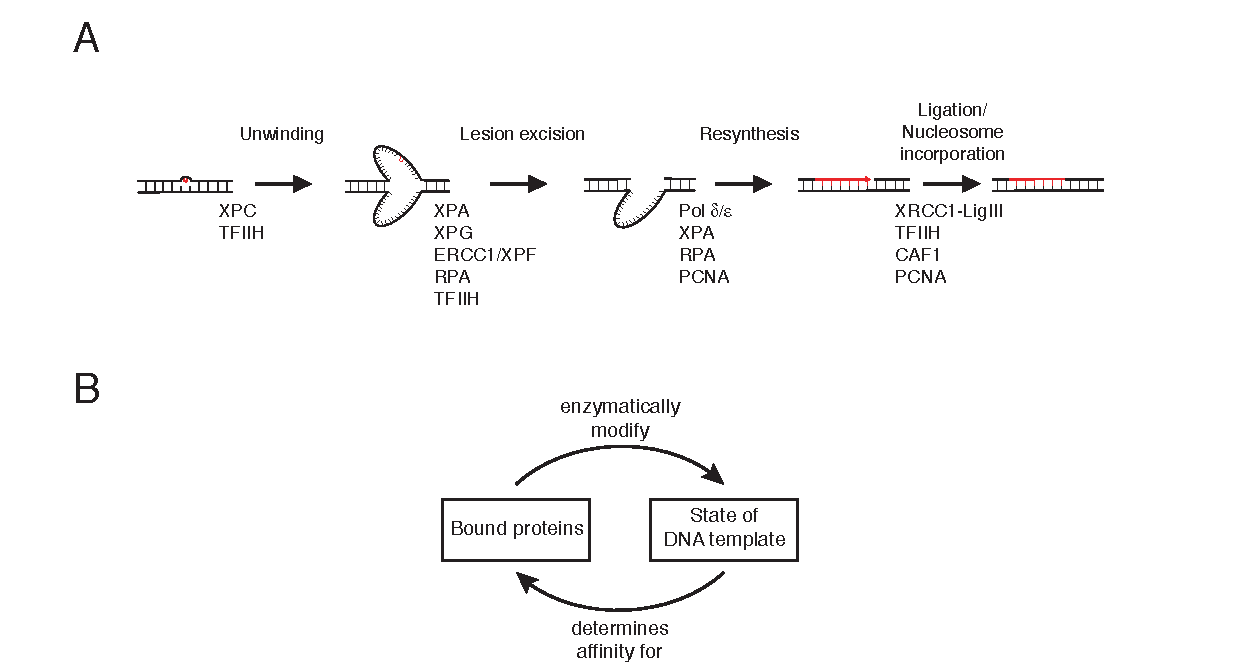
\includegraphics[width=1\textwidth]{Abbildungen/figure1_1.pdf}
		\caption{\textbf{NER as a paradigm for chromatin-associated processes.} A) Graphical scheme of the NER pathway. Shown is the sequence of repair intermediates together with the repair factors that, if fully assembled, catalyse the next reaction. B) 'Recruiting-reaction' cycle illustrating the principle of the sequential organization of chromatin-associated processes. Therein, recruited process components catalytically modify the DNA template and thereby redefine the binding affinity for the next complex.}
		\label{fig:introScheme}
	\end{center}
\end{figure} 

\paragraph{Data-driven kinetic modelling of NER}
Defects in GG-NER are associated with the prototypical nucleotide-excision-repair disorder xeroderma pigmentosum (XP), which is associated with pigmentation abnormalities and an increased risk of skin cancer and internal tumours \cite{Hoeijmakers2009}. XP is caused by gene-defects in one of the seven XP-genes, XPA through XPG. Despite the severe symptoms related to one of these defects all patients are viable, which allowed for the isolation of patient cell lines where the endogenous NER factor is knocked-out. More importantly, these cell lines could be transfected with a GFP-tagged construct of the missing protein enabling the fluorescence real-time measurement of the NER factor kinetics \cite{Hoogstraten2002,Hoogstraten2008,Zotter2006,Rademakers2003}. Taken together, the clearly defined UV-mediated inducibility of NER combined with the availability of the fluorescently-tagged core repair factors makes NER a paradigm for the research on chromatin-associated processes.\\
On the basis of accumulation and dissociation time courses for each NER factor Luijsterburg \textit{et.\ al.}\cite{Luijsterburg2010} developed a quantitative model of the NER process. This model suggests for the formation of enzymatically active protein complexes a cyclic principle (cf.\ Figure \textbf{tbm}B): Repair factors bind reversibly and assemble stochastically at the DNA template; once the complex is fully assembled it modifies the DNA substrate and thereby changes the binding affinity for the next enzymatic complex. Traversing multiple of these 'recruiting-reaction' cycles will translate the recurring stochastic protein exchange at the chromatin site into an ordered sequence of regulatory events \cite{Dinant:2009:J-Cell-Biol:19332890}.\\
This model unravels a number of interesting relations between assembly dynamics and process functionality, \textit{e.g.} that rapidly reversible protein binding allows for high specificity of the pathway through kinetic proofreading \cite{Luijsterburg2010}. In agreement to this notion, such combinations of live cell experiments and mathematical modelling have led to equally intriguing results for transcription. As indicated by Gorski \textit{et.\ al.} \cite{Gorski:2008:Mol-Cell:18498750} already a moderate increase in the dwell-time of RNA Pol I subunits caused the enhancement of the assembly efficiency and the initiation rate of RNA Pol I. Another study describes a mechanism termed 'assisted loading', where a weak transcription factor-DNA interaction facilitates the binding of a second transcription factor and thereby obviates the need for simultaneous and cooperative binding \cite{Voss2011}. \\         
A prevailing problem affecting the value of quantitative model predictions is concerned with the non-identifiability of the model parameters by the \textit{in vivo} data (on-rate and off-rate constants as well as enzymatic rate constants). As a consequence the parameter uncertainties are propagated to the model predictions, which limits their significance \cite{Raue2013}. To overcome these limitations further developments in the model-driven analysis of chromatin-associated processes will depend on the integration of model calibration, uncertainty analysis and experimental design.     
  

\section{Research objectives}

In the course of this study, we want to expand the theoretical analysis of the NER process and thereby increase our understanding of the interrelation between protein-complex assembly dynamics and the functionality of chromatin-associated machineries. This analysis will be guided by the following questions:

\begin{itemize}
	\item What is the quantitative relation between the 'recruitment-reaction' design principle of functional repair complexes and the overall repair kinetic of the DNA lesions?
	
	\item Which pathway components contribute to the control of the apparent repair rate? 
	
	\item Which molecular mechanisms are responsible for the robust regulation of DNA repair? 
\end{itemize} 

To start with, we extended the comprehensive information about protein dynamics measured previously with a time-resolved readout of DNA repair synthesis in individual living cells. The measured time course follows a slow first-order kinetic, which turned out to be compatible with the current understanding of rapidly reversible protein assembly. With the combined data set we were able to identify a realistic model of NER and thus to make quantitative predictions about the repair process. One particularly captivating model outcome disagrees with the existence of a rate-limiting repair factor but instead emphasises a shared and moderate control of the repair rate. Exploiting the natural variability in repair factor expression we found experimental support for this prediction. Intriguingly, the protein expression itself is correlated independent of the repair process and the cell cycle stage. This suggests that the robustness of DNA repair is regulated by a combination of collective NER factor rate control and a so far unknown pre-transcriptional mechanism.\\   

This work has been conceived and carried out in close collaboration with Dr. Paul Verbruggen and Prof. Emer. Roel van Driel (University of Amsterdam).





